% Options for packages loaded elsewhere
\PassOptionsToPackage{unicode}{hyperref}
\PassOptionsToPackage{hyphens}{url}
%
\documentclass[
]{article}
\usepackage{lmodern}
\usepackage{amssymb,amsmath}
\usepackage{ifxetex,ifluatex}
\ifnum 0\ifxetex 1\fi\ifluatex 1\fi=0 % if pdftex
  \usepackage[T1]{fontenc}
  \usepackage[utf8]{inputenc}
  \usepackage{textcomp} % provide euro and other symbols
\else % if luatex or xetex
  \usepackage{unicode-math}
  \defaultfontfeatures{Scale=MatchLowercase}
  \defaultfontfeatures[\rmfamily]{Ligatures=TeX,Scale=1}
\fi
% Use upquote if available, for straight quotes in verbatim environments
\IfFileExists{upquote.sty}{\usepackage{upquote}}{}
\IfFileExists{microtype.sty}{% use microtype if available
  \usepackage[]{microtype}
  \UseMicrotypeSet[protrusion]{basicmath} % disable protrusion for tt fonts
}{}
\makeatletter
\@ifundefined{KOMAClassName}{% if non-KOMA class
  \IfFileExists{parskip.sty}{%
    \usepackage{parskip}
  }{% else
    \setlength{\parindent}{0pt}
    \setlength{\parskip}{6pt plus 2pt minus 1pt}}
}{% if KOMA class
  \KOMAoptions{parskip=half}}
\makeatother
\usepackage{xcolor}
\IfFileExists{xurl.sty}{\usepackage{xurl}}{} % add URL line breaks if available
\IfFileExists{bookmark.sty}{\usepackage{bookmark}}{\usepackage{hyperref}}
\hypersetup{
  hidelinks,
  pdfcreator={LaTeX via pandoc}}
\urlstyle{same} % disable monospaced font for URLs
\usepackage{graphicx}
\makeatletter
\def\maxwidth{\ifdim\Gin@nat@width>\linewidth\linewidth\else\Gin@nat@width\fi}
\def\maxheight{\ifdim\Gin@nat@height>\textheight\textheight\else\Gin@nat@height\fi}
\makeatother
% Scale images if necessary, so that they will not overflow the page
% margins by default, and it is still possible to overwrite the defaults
% using explicit options in \includegraphics[width, height, ...]{}
\setkeys{Gin}{width=\maxwidth,height=\maxheight,keepaspectratio}
% Set default figure placement to htbp
\makeatletter
\def\fps@figure{htbp}
\makeatother
\setlength{\emergencystretch}{3em} % prevent overfull lines
\providecommand{\tightlist}{%
  \setlength{\itemsep}{0pt}\setlength{\parskip}{0pt}}
\setcounter{secnumdepth}{-\maxdimen} % remove section numbering

\author{}
\date{}

\begin{document}

\hypertarget{asip-meister}{%
\section{ASIP Meister}\label{asip-meister}}

ASIP Meister {[}ASIPMeister{]} is a development environment for creating
application specific instruction set processors (ASIPs). It is not the
purpose of this chapter to explain the benefits or the usage of ASIP
Meister. To learn the usage of ASIP Meister you have to work through the
user manual and the tutorial, which are available in the ``share''
subdirectory of ASIP Meister. ASIP Meister itself is located in the
directory /AM/ASIPmeister/ in our laboratory environment. The purpose of
this chapter is to summarize some typical challenges with ASIP Meister
and some typical but hard to understand error messages, that might
appear while using the software. Chapter~4.4 will afterwards give a
tutorial about the so-called `Flexible Hardware Model' (FHM) of ASIP
Meister, as this part is missing in the official tutorial.

\hypertarget{what-is-asip-meister}{%
\subsection{What is ASIP Meister?}\label{what-is-asip-meister}}

ASIP Meister is a tool for developing Application Specific Instruction
Set Processors (ASIPs) from high level specification description. The
functionality of the tool is listed below:

\begin{itemize}
\item
  Automatic generation of the processor HDL description from Micro Op.
  description.
\item
  Fast Estimation of processor design quality at an early stage of
  design process.
\end{itemize}

%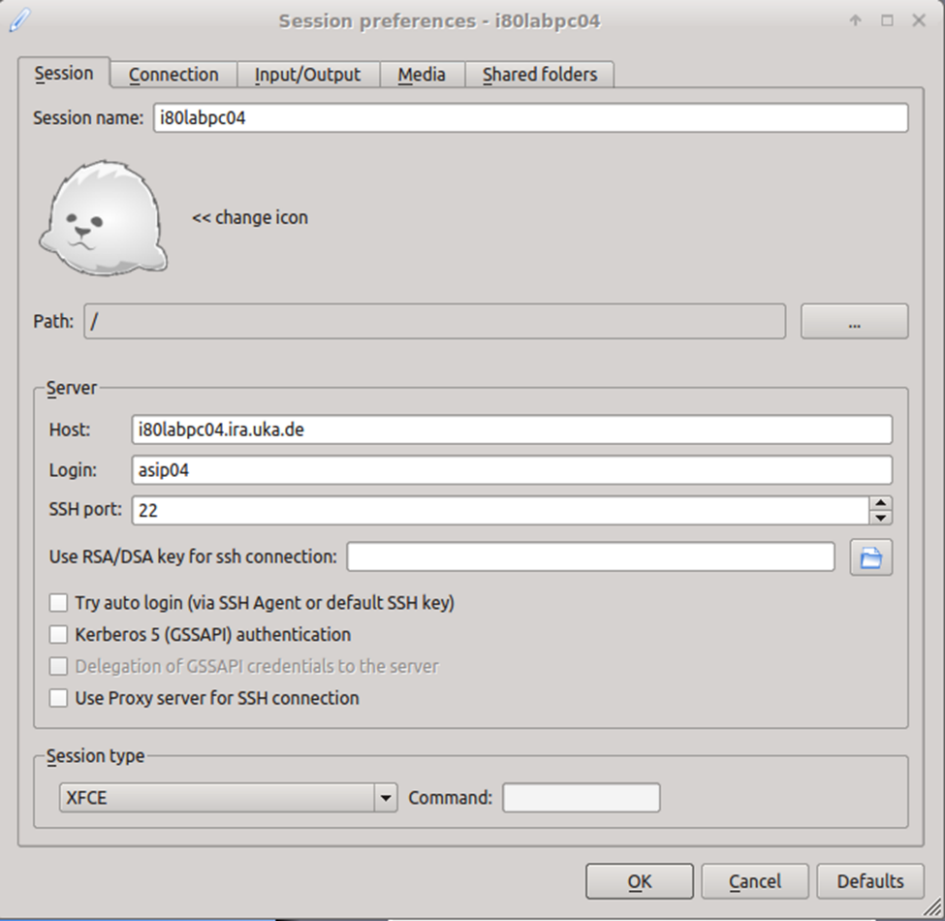
\includegraphics[width=5.5038in,height=3.52185in]{media/image1.png}
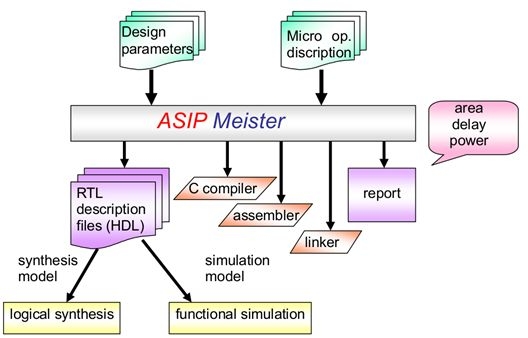
\includegraphics[width=6.09196in,height=3.97917in]{4-1.png}
Figure 4‑1: ASIP Meister Input and Output

For the above functionality, it is possible to examine and compare
different architecture implementations using ASIP Meister. The
input/output of ASIP Meister is roughly shown in the figure below. Using
the GUI of ASIP Meister, the user inputs the design parameters and Micro
Op. description. ASIP Meister generates an estimation report of the
processor design quality and its RTL description files. Furthermore,
ASIP Meister also generates a development environment composed of a C
compiler, assembler and linker. The synthesis model and the simulation
model are automatically generated in HDL. These models then become the
input to logical synthesis tools and functional simulation tools.

\hypertarget{processor-design-flow-using-asip-meister}{%
\subsection{Processor Design Flow Using ASIP
Meister}\label{processor-design-flow-using-asip-meister}}

Open each sub-window in ASIP Meister, in the order specified in Figure
4-2. This would be typically the order of operation that should be
performed to design and generate a processor core using ASIP Meister.

%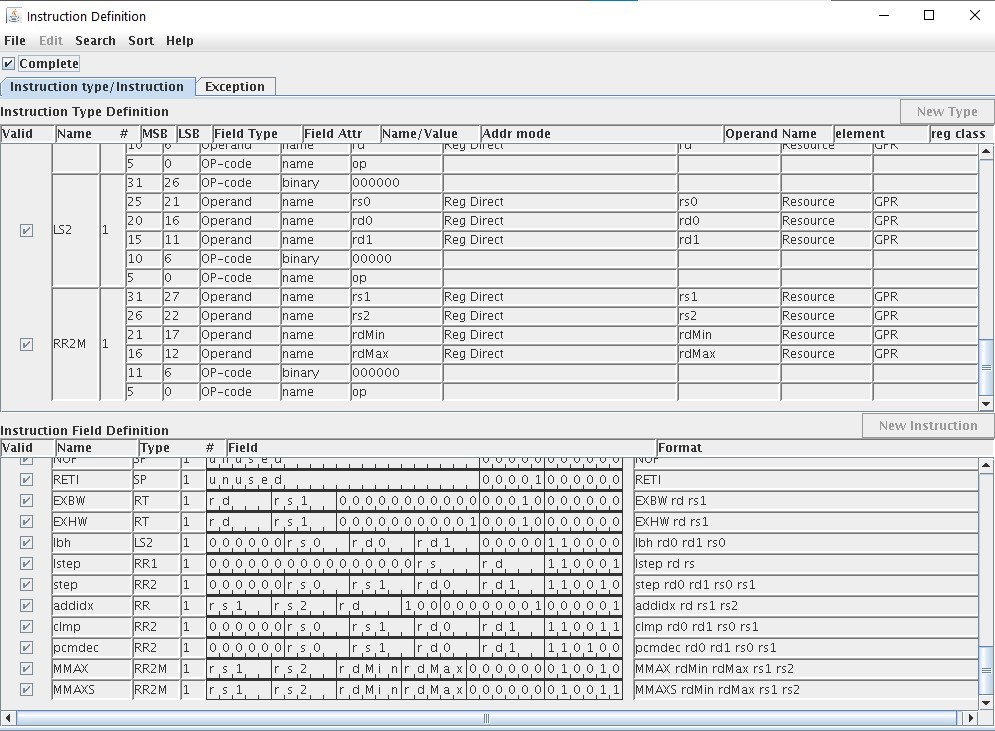
\includegraphics[width=6.29444in,height=3.35208in]{media/image2.jpg}
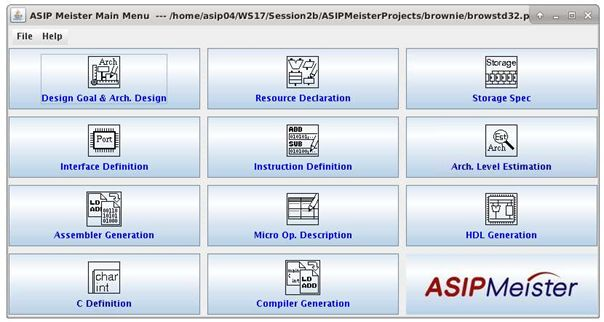
\includegraphics[width=6.09196in,height=3.97917in]{4-2.png}
Figure 4‑2: ASIPmeister main window

1. \textbf{Design Goal \& Arch. Design}: Setting design goal values and
pipeline stages

2. \textbf{Resource Declaration}: Declaring resources

3. \textbf{Storage Specification}: Definition Specifying storages

4. \textbf{Interface Definition}: Defining I/O interfaces of the target
processor

5. \textbf{Instruction Definition}: Defining instruction types and
instruction set

6. \textbf{Arch. Level Estimation}: Estimating design quality of target
processor

7. \textbf{Assembler Generation}: Generating Assembler description files

8. \textbf{Micro Op. Description}: Describing micro-operations for each
instruction

9. \textbf{HDL Generation}: Generating HDL files of target processor

10. \textbf{C Definition}: Defining C code

11. \textbf{Compiler Generation}: Generating compiler and Binutils

For details of the individual sub-windows, see the corresponding
sections in {[}TUT{]} and {[}UM{]}.

\hypertarget{typical-challenges-while-working-with-asip-meister}{%
\subsection{Typical Challenges while Working with ASIP
Meister}\label{typical-challenges-while-working-with-asip-meister}}

\begin{itemize}
\item
  The \textbf{register r0} is hardwired to zero in our ASIP Meister CPU.
  Nevertheless, this is only a hint for the compiler. The compiler will
  never try to write a value different from zero to this register and
  the compiler will use this register when a zero value is needed.
  However, this register can be written with any value, like all the
  other registers. The reason for this behavior is that the register
  file is created by the FHM description (flexible hardware model) in
  the ``\emph{Resource Declaration}'', and the configurations in the
  ``\emph{Storage Specifications}'' are only used for the compiler and
  assembler, but are not used for creating the hardware.
\item
  Do not use the ``\emph{meister/xxx.sim}'' directory like
  ``\emph{browstd32.sim}'', when simulating or synthesizing the VHDL
  code. There is a problem with the register file. Instead, use the
  ``\emph{meister/xxx.syn}'' directory like ``\emph{browstd32.syn}''.
  The same VHDL-code will be used for synthesis as explained in
  Chapter~6.
\item
  ASIP Meister can only be used once on each computer. Therefore, if two
  different groups want to work with ASIP Meister, they have to use
  different computers. To make sure, that ASIP Meister is at most
  started once on each PC, the starting script tests, whether the file
  ``\textbf{/tmp/fhm\_server.log}'' exists in the temporary directory.
  ASIP Meister creates this file while starting and it is removed after
  ASIP Meister terminates. If this file exists, then someone else might
  already use ASIP Meister on that PC. However, it can also happen, that
  this file is not automatically deleted, after ASIP Meister terminates.
  If you think, that no one else is using ASIP Meister on this PC, then
  remove this file.
\item
  When writing \textbf{MicroOp} code, be careful with macros. A macro
  that is defined as three stage long and started in the ID phase will
  execute in the ID, the EX and the MEM phases, not just in the ID
  phase. If you want to view an instruction's \emph{MicroOp} code
  without macros, select this instruction and hit the ``\emph{Macro
  Expansion}'' button in the upper right corner.
\end{itemize}

\hypertarget{tutorial-for-the-flexible-hardware-model-fhm}{%
\subsection{Tutorial for the ``Flexible Hardware Model''
(FHM)}\label{tutorial-for-the-flexible-hardware-model-fhm}}

To add a new instruction to an ASIP Meister CPU one would usually write
a \emph{MicroOp} description for the instruction, using the facilities
of an existing hardware module (ALU, shifter, adder, etc.) The ability
to use multiple hardware modules during one stage and to create more
than one instance of a specific module combined with the operators
provided by the \emph{MicroOp} description language is sufficient for
most basic instructions. However, this method has several shortcomings
that make it impossible to do the following (among others):

\begin{itemize}
\item
  Working with not program-defined wire ranges which depend on register
  contents or immediate values
\item
  Implementing multi-cycle instructions
\end{itemize}

This tutorial will show how to write a new hardware module to provide a
"\emph{rotate left}" instruction.

\hypertarget{setting-up-asip-meister-to-add-new-fhm}{%
\subsubsection{Setting up ASIP Meister to add new
FHM}\label{setting-up-asip-meister-to-add-new-fhm}}

In our current setup, ASIP Meister is installed globally. To modify FHMs
you will need to set it up locally:

\begin{enumerate}
\def\labelenumi{\arabic{enumi}.}
\item
  Copy the ASIP Meister directory tree to your home directory:
\end{enumerate}

\begin{quote}
cp -r /AM/ASIPmeister// \textasciitilde{}
\end{quote}

\begin{enumerate}
\def\labelenumi{\arabic{enumi}.}
\setcounter{enumi}{1}
\item
  Update the PATH environment variable to use the local ASIP Meister
  directory by editing the file \emph{\textasciitilde/.bashrc.user} and
  adding the following line at the end of the file:
\end{enumerate}

\begin{quote}
PATH=\$HOME/ASIPmeister/bin/:\$PATH
\end{quote}

\begin{enumerate}
\def\labelenumi{\arabic{enumi}.}
\setcounter{enumi}{2}
\item
  Force the shell to re-read the \emph{bashrc} file to use the updated
  PATH variable:
\end{enumerate}

\begin{quote}
source \textasciitilde/.bashrc or logout and login again
\end{quote}

\begin{enumerate}
\def\labelenumi{\arabic{enumi}.}
\setcounter{enumi}{3}
\item
  Verify that you are using the correct ASIP Meister copy: \emph{``which
  ASIPmeister''} should print the path to the local copy
\item
  Edit \emph{\textasciitilde/ASIPmeister/bin/ASIPmeister} (line 25) and
  make sure your local ASIP Meister path (\emph{\$HOME/ASIPmeister}) is
  assigned to the variable \emph{ASIP\_MEISTER\_HOME}.
\end{enumerate}

From now on whenever relative paths (not starting with a /) are
mentioned, \emph{\$HOME/ASIPmeister} should be the base directory, i.e.:
\emph{share/­fhmdb/­workdb/­peas/­rotator.fhm} should be
/\emph{home/­asipXX/­ASIPmeister/­share/­fhmdb/­workdb/­peas/­rotator.fhm}

\hypertarget{fhm-structure}{%
\subsubsection{FHM structure}\label{fhm-structure}}

The directory \emph{share/fhmdb} has two subdirectories and the file
\emph{fhmdbstruct}. ASIP Meister reads this file to determine which FHM
files to use. Most of the modules necessary for the basic functions of
the CPU are in the directory \emph{basicfhmdb}; they are further divided
into the categories \emph{computational} and \emph{storage}. New FHMs
should be added to the \emph{share/­fhmdb/­workdb/­peas} directory.

FHMs are written in XML (eXtensible Markup Language). ASIP Meister
processes their data in several stages, most importantly ``\emph{HDL
Generation''} which creates the CPU VHDL files. Usually some embedded
Perl is used in the FHMs to customize VHDL code. An FHM can be divided
roughly into two parts: \emph{behavior} and \emph{synthesis}. We are not
going to differ between them, though.

\textbf{Header and Function description}

First, we need to make ASIP Meister aware of our new FHM. Edit
\emph{share/­fhmdb/­fhmdbstruct}. Go to the tag \emph{\textless library
name="workdb"\textgreater{}} and add another model to the peas class by
adding the line
\emph{\textless model\textgreater rotator\textless/model\textgreater{}}.
Save and close the file, as this is the only change needed for this
file.

To make your task a bit easier, we have prepared a template file with
many mandatory sections already done. Copy the file
\emph{share/fhmdb/workdb/peas/skeleton-1p.fhm} to
\emph{share/fhmdb/workdb/peas/rotator.fhm} and edit this file. TAKE
CARE: Small errors in this file will lead to very general error messages
that are hard to find. Consider the general hint in Chapter~4.6 and
double-check your changes for typing errors and missing spaces.

Name your FHM ``\emph{rotator}'' by editing the name in the
\emph{\textless model\_name\textgreater{}} tag. Rename the author in the
\emph{\textless author\textgreater{}} tag. The
\textless parameter\textgreater{} section is used to allow FHM
customization from the \emph{Resource declaration} section in ASIP
Meister. The parameter \emph{bit\_width} for the input and output vector
is already defined. Leave it as it is.

Next, we have the \emph{function description}, which is generated with
an embedded Perl script. Functions are used by ASIP Meister to interface
the MicroOp description and the actual VHDL code. The program generates
the necessary registers/multiplexers and control signals to address the
corresponding hardware module. The Perl script uses the Perl
\emph{print} function to output the \emph{function description}. The
\emph{\textless\textless{}} and the following string start a so called
``\emph{here document''}, which instructs the Perl interpreter to treat
all the following lines as single character string (performing variable
substitution) until it finds the string after the
\emph{\textless\textless{}} on a single line.

Rename the name of the \emph{function} from "\emph{foo}" to
"\emph{rotl}" and change the comment in the line above to something
sensible (e.g. "\emph{rotate left}").

Functions are divided into 4 blocks:

\textbf{input:} declaration of \emph{function parameters}. We need the
actual data and the amount by which to rotate, so write the following
two lines between the curly braces of \emph{input}:

bit {[}\$msb:0{]} data\_in;

bit {[}7:0{]} amount;

\begin{quote}
Note that \emph{\$msb} is a Perl variable that will be substituted by
the actual value (assigned above, \emph{\$bit\_width - 1})
\end{quote}

\textbf{output:} declaration of the \emph{function output}. The rotated
value is of the same type as the input value, so add the following
between the braces of the \emph{output} block:

bit {[}\$msb:0{]} data\_out;

\textbf{control:} \emph{control variables} used by the RTG controller of
the CPU. These signals are not accessible from the MicroOp description,
but can be used in the VHDL code in the FHM. For our hardware to know
which direction (left or right) to shift, we will use a 1 bit signal
('0' for left, '1' for right). Add the following for the \emph{control}
section:

in direction;

\begin{quote}
The \emph{in} keyword means that the module will be able to access the
signal read-only. \emph{out} and \emph{inout} are the other two
possibilities.
\end{quote}

\textbf{protocol:} Describes what the \emph{function} should do once a
condition is met. In this case, we will use the following simple
protocol:

{[}direction == '0'{]} \{

valid data\_out;

\}

That is, it is for the \emph{function description}. The \emph{function
convention} is next. The content is identical to the \emph{function
description} except for the following two changes:

\emph{Write the following into the protocol} block:

single\_cycle\_protocol \{

direction = '0';

\}

Write the following into the \emph{control} block:

in bit direction;

To declare additional \emph{functions}, simply add their descriptions to
the ``\emph{here document}'' (or use a new print statement), do not
start a new XML \emph{\textless function\_description\textgreater{}} or
\emph{\textless function\_conv\textgreater{}} block.

\textbf{Ports, Instance and Entity}

The \emph{\textless function\_port\textgreater{}} section declares the
signals that will be connected to our module. As with the \emph{function
convention} and \emph{function description} it is an embedded Perl
script, and as before the output is done with the ``\emph{here
document''}. We mentioned all the needed ports in the \emph{function
convention} and \emph{description} already: \emph{direction},
\emph{data\_in}, \emph{amount}, \emph{data\_out}. Use the following
lines for the declaration (make sure you write them between the
``\emph{print \textless\textless FHM\_DL\_PORTS;''} and the
``\emph{FHM\_DL\_PORTS lines}'' in the
\emph{\textless function\_port\textgreater{}} part):

direction in bit mode

data\_in in bit\_vector \$msb 0 data

amount in bit\_vector 7 0 data

data\_out out bit\_vector \$msb 0 data

You will notice two things: First, there are two types of ports: mode
and data ports\footnote{There is another type: ctrl which is used for
  multi cycle instructions} - use \emph{data} for your input and output
signals and \emph{mode} for control signals. Second, one bit signals are
declared as bit and don't have a range specification, while signals
wider than one bit (vectors) are of type \emph{bit\_vector} and have a
range (width) - in this case from the most significant bit down to 0.

The \emph{\textless instance\textgreater{}} is the core of the module -
the actual architecture VHDL code. Embedded Perl is used here as well.
Go to the \emph{\$signals} variable. As you can see here, documents can
also be used to assign values to variables. No additional signals are
necessary for our rotator, so we will leave \emph{\$signals} as it is.

The next variable, \emph{\$vhdl} is more interesting: Our module should
be sensitive to changes of input data, shifting amount and shifting
direction (so it should re-compute the output data if one of these three
values changes), hence we define a process with these three values in
its sensitivity list. We also need one integer variable to hold the
value of the shifting amount (\emph{amount} is a signal, not a variable)
and one signal for the temporary value of the result. After the
\emph{begin} keyword we can write the process code. Remember that this
variable (as all the others) will later be used to create the actual
VHDL output (the variable is not placed at the correct position for the
VHDL output, but instead it is later used at the correct position). If
you are writing statements that span multiple lines you have to
encapsulate them with double quotes (``\,'') to assign them to the
variable.

First, we need to convert the signal \emph{amount} to integer and assign
it to \emph{a}. Next we check if \emph{a} is within range, if it is not,
we set the result to \emph{undefined}, otherwise we can rotate. A case
switch is used to decide into which direction to rotate. The
\emph{others} case is necessary, as the type \emph{std\_logic} has more
states than just '0' and '1', so don't delete it when you add the code
for "rotate right".

At the end of the process, we assign the value of the \emph{res} signal
to the \emph{data\_out} signal. See below listing for the architecture
VHDL:

process (data\_in, amount, direction)

variable a : integer;

variable res : std\_logic\_vector(\$msb downto 0);

begin

a := TO\_INTEGER(UNSIGNED(amount));

if (a \textgreater{} 0 and a \textless{} \$bit\_width) then

case direction is

when '0' =\textgreater{} -\/- rotate left

res(\$msb downto a) :=

data\_in(\$msb - a downto 0);

res(a - 1 downto 0) :=

data\_in(\$msb downto \$bit\_width - a);

when others =\textgreater{} -\/- not reached

res := (others =\textgreater{} 'X');

end case;

else

res := (others =\textgreater{} 'X');

end if;

data\_out \textless= res;

end process;

Leave the comment section untouched and look closer at the
FHM\_DL\_TOP\_2 document. First, three libraries are included - these
are necessary for the std\_logic data types and several functions and
macros. Next, the entity is declared, which states all input and output
ports of our VHDL module. Although we already defined the ports of our
FHM, these were interpreted by ASIP Meister - the port declaration for
the entity, as well as the rest of the VHDL code will be used verbatim,
without any error checking by ASIP Meister (although we can still check
for errors in ModelSim). Use the code in the below listing (between the
``\emph{print \textless\textless FHM\_DL\_PORTS;''} and the
``\emph{FHM\_DL\_PORTS lines}'' in the
\emph{\textless instance\textgreater{}} part) for the entity ports:

data\_in : in std\_logic\_vector(\$msb downto 0);

direction : in std\_logic;

amount : in std\_logic\_vector(7 downto 0);

data\_out : out std\_logic\_vector(\$msb downto 0)

That is for the \emph{\textless instance\textgreater{}} block. Next, we
have an \emph{\textless entity\textgreater{}} section. It defines an
\emph{entity} in a different file, which is why a new block is needed,
but the ports are the same, so use the code from the above listing.

\hypertarget{estimation-and-the-synthesis-model}{%
\subsubsection{Estimation and the Synthesis
Model}\label{estimation-and-the-synthesis-model}}

The \emph{\textless testvector\textgreater{}} section may be left empty,
the \emph{\textless synthesis\textgreater{}} script contains
instructions to process the FHM file - we leave that untouched as well.

The \emph{\textless estimation\textgreater{}} block has data relevant
for area, power and delay estimations, but we use more accurate tools,
that consider the actual application execution, as shown in Chapter~6.5,
and Chapter~7.2. Leave the estimation data there though, as ASIP Meister
will complain without them. You should change FHM parameters however,
you will have to adjust the estimation section if you want to get rid of
the warnings.

That is it for the \emph{behavior} model. As mentioned in the beginning,
we won't differ between the \emph{behavior} and the \emph{synthesis}
model, so just copy-and-paste the complete
\emph{\textless model\textgreater{}} block and change the value of the
\emph{\textless design\_level\textgreater{}} tag from behavior to
synthesis.

Your FHM file should now have a structure similar to the following
listing:

\textless?xml version="1.0" encoding="Shift\_JIS" ?\textgreater{}

\textless FHM\textgreater{}

\textless model\_name\textgreater{} rotator
\textless/model\_name\textgreater{}

\textless model\textgreater{}

\textless design\_level\textgreater{} behavior
\textless/design\_level\textgreater{}

{[}...{]}

\textless/model\textgreater{}

\textless model\textgreater{}

\textless design\_level\textgreater{} synthesis
\textless/design\_level\textgreater{}

{[}...{]}

\textless/model\textgreater{}

\textless/FHM\textgreater{}

You can now use the module in ASIP Meister. Instantiate the FHM resource
in the \emph{Resource Declaration} and write the new instruction
\emph{rotl}. Set the operands to the correct Addressing Mode, DataType,
etc in the \emph{Behavior Description} window, but leave the behavior
description itself out. Use the syntax

result = ROT0.rotl(source0, am);

where \emph{result} and \emph{source0} are 32-bit wires and \emph{am} is
a 8-bit wire.

\hypertarget{testing-the-new-fhm}{%
\subsubsection{Testing the new FHM}\label{testing-the-new-fhm}}

When HDL and SWDev Generation run without errors (SWDev will probably
print some warnings about setting throughput to 1 - that is alright),
proceed testing your module/instruction. Write a small assembly code,
compile it (as shown in \protect\hyperlink{Fig22}{Figure 2-2}), create a
new project in ModelSim, load your design and compile it. If there are
errors during compilation of the VHDL files (especially in
\emph{fhm\_rotator\_w32.vhd)}, then you have made a mistake in your VHDL
code. Now you could go back to the FHM and correct it there, but a
faster way is to edit the mentioned VHDL file in your
\emph{\textasciitilde/ASIPMeisterProjects/­browstd32\_YourCPU/­meister/­browstd32\_YourCPU.syn/}
directory and try to correct the code there. Once you get it running,
make the corrections in the FHM file as well (important: in the behavior
{and} synthesis sections), as ASIP Meister will overwrite the VHDL files
every time you recreate the CPU.

Once your CPU VHDL files are compiled, run your test program. Check the
results carefully! Experiment with large values as well (i.e. use
\emph{lhi \%r2, \$65535} to set the upper 16 bits to '1'). Once you
verified your design, backup your FHM (important!) and implement the
``\emph{rotr} `` - right rotation instruction by making the necessary
changes to your FHM.

\hypertarget{multi-cycle-fhms}{%
\subsection{Multi Cycle FHMs}\label{multi-cycle-fhms}}

As mentioned at the beginning of the tutorial, one of the reasons to
write custom FHMs is to implement multi-cycle (stalling) instructions.
Examples of stalling instructions are the multiplication and division
operations, which use dedicated multiplier and divider hardware blocks.
Stalling hardware is usually implemented with \emph{State Machines}.
This section will show you how to write a FHM for a multi-cycle
instruction. We will extend the rotator from the previous sections - the
multi-cycle version will rotate only one bit per cycle (obviously the
performance will be inferior to the single-cycle variant; it is just for
demonstration).

ASIP Meister provides three signals to control multi-cycle instructions:
\emph{start}, \emph{fin} and \emph{cancel}. The \emph{start} signal will
be set by the RTG controller once the instruction is started, and our
hardware will set the \emph{fin} signal once the operation is finished,
to signal the CPU that normal pipeline operation can be resumed. If a
\emph{cancel} signal arrives, the hardware should abort its operation.
We will disregard the cancel signal here, but reset our hardware on the
CPU \emph{reset} signal into its default state.

\textbf{\textless function\_description\textgreater{}}

We need to define the three control signals in the \emph{control} block
of our function. As the \emph{control} block of your function use

in start, cancel, direction;

out fin;

We also need a protocol for our stalling instruction. For the
\emph{protocol} block use:

repeat {[}start == 1{]} until (fin == 1 \textbar\textbar{} cancel == 1);

if (fin == 1 \&\& direction == 0) \{

valid data\_out;

\}

\textbf{\textless function\_conv\textgreater{}}

Add the three signals to the \emph{control} block of your function. It
should be now:

in bit direction;

in bit start;

in bit cancel;

out bit fin;

and for the \emph{protocol} block use:

multi\_cycle\_protocol \{

start\_signal start = '1';

fin\_signal fin = '1';

cancel\_signal cancel = '1';

direction = '0';

\}

\textbf{\textless function\_port\textgreater{}}

The three signals as well as the CPU \emph{clock} and \emph{reset}
signals need to be added to the port declaration of our FHM, so use:

direction in bit mode

data\_in in bit\_vector \$msb 0 data

amount in bit\_vector 7 0 data

data\_out out bit\_vector \$msb 0 data

clock in bit clock

reset in bit reset

start in bit ctrl

fin out bit ctrl

cancel in bit ctrl

Note that the port type is \emph{ctrl}, not \emph{mode} for the three
multi-cycle control signals, and \emph{clock} and \emph{reset} for the
two CPU signals respectively.

\textbf{\textless instance\textgreater{}}

The VHDL implementation uses one process for the state machine, but this
time we only use \emph{clock} and \emph{reset} in its sensitivity list.
In the process body, we first handle the reset case (synchronously), and
then depending on the current state we either start the state machine
from the idle state (\emph{st0}), execute a one-bit rotation
(\emph{st1}), or assign the result (\emph{st2}). The following code is
provided as text file as well:

\$vhdl = "process (clock, reset)

type t\_s is (st0, st1, st2);

variable state : t\_s;

variable a : integer;

variable res : std\_logic\_vector(\$W1 downto 0);

variable tmp\_data : std\_logic\_vector(31 downto 0);

begin

if rising\_edge(clock) then

-\/- handle reset (synchronous)

if reset = '1' then

state := st0;

data\_out \textless=
\textbackslash"00000000000000000000000000000000\textbackslash";

fin \textless= '1';

else

case state is

when st0 =\textgreater{}

if start = '1' then

state := st1;

a := TO\_INTEGER(UNSIGNED(amount));

tmp\_data := data\_in;

end if;

fin \textless= '0';

when st1 =\textgreater{}

if (a \textgreater{} 0 and a \textless{} \$bit\_width) then

case direction is

when '0' =\textgreater{} -\/- rotate left one bit

res(\$W1 downto 1) := tmp\_data(\$W1 - 1 downto 0);

res(0) := tmp\_data(\$W1);

when others =\textgreater{} -\/- not reached

res := (others =\textgreater{} 'X');

end case;

a := a - 1;

tmp\_data := res;

else

if a /= 0 then

res := (others =\textgreater{} 'X');

end if;

state := st2;

end if;

fin \textless= '0';

when st2 =\textgreater{}

data\_out \textless= res;

state := st0;

fin \textless= '1';

end case;

end if;

end if;

end process;";

Further down, in the \emph{entity} declaration, we will need to add our
three control signals as well as the clock and reset signals. The entity
should now have the following signals:

data\_in : in std\_logic\_vector(\$W1 downto 0);

direction : in std\_logic;

amount : in std\_logic\_vector(7 downto 0);

data\_out : out std\_logic\_vector(\$W1 downto 0);

clock : in std\_logic;

reset : in std\_logic;

start : in std\_logic;

cancel : in std\_logic;

fin : out std\_logic);

\textbf{\textless entity\textgreater{}}

Again, our five signals need to be added to the \emph{entity}
declaration. The new \emph{entity} should have:

data\_in : in std\_logic\_vector(\$W1 downto 0);

direction : in std\_logic;

amount : in std\_logic\_vector(7 downto 0);

data\_out : out std\_logic\_vector(\$W1 downto 0);

clock : in std\_logic;

reset : in std\_logic;

start : in std\_logic;

cancel : in std\_logic;

fin : out std\_logic);

\hypertarget{estimation-synthesis-asip-meister-usage-and-testing}{%
\subsubsection{Estimation, Synthesis, ASIP Meister usage and
Testing}\label{estimation-synthesis-asip-meister-usage-and-testing}}

No changes for estimation or synthesis but make sure to copy your
changes to the behavior \emph{\textless model\textgreater{}} section of
the FHM.

Instantiate and use the resource in ASIP Meister just as with a
singly-cycle FHM - no changes needed. Write a test program and check in
ModelSim whether the pipeline actually stalls (the \emph{im\_addr} value
shouldn't change during stalling) and whether the result is the same as
with the single-cycle instruction.

\hypertarget{general-hints-about-fhms}{%
\subsection{General Hints about FHMs}\label{general-hints-about-fhms}}

\begin{itemize}
\item
  Do not copy and paste the code from this \emph{pdf} file. Often, this
  manifests in wrong code (e.g. wrong blanks) and the effort to debug
  the code afterwards is bigger, than manually transcribing the code.
\item
  ASIP Meister has only very few debug facilities for FHMs (e.g.
  \emph{/tmp/fhm\_server.log} contains some more information compared to
  the popup windows). Therefore, you usually have to use the trial and
  error scheme. The syntax for FHMs is very restrictive. Sometimes a
  missing blank can cause a problem. Sometimes (!) you can ignore error
  messages in the \emph{Resource Declaration}, as long as the resource
  was successfully instantiated. These error messages are meant for the
  \emph{Estimation,} which is not needed for the implementation.
\item
  The FHM example in this tutorial is constructed for a module with one
  parameter. When you need more parameters, have a look at the other
  existing FHMs.
\item
  As soon as a new FHM is successfully constructed, you can make further
  changes directly in the VHDL code for simplicity. Whenever the VHDL
  code is finalized, you should include it into the FHM file again, as
  the created VHDL files are overwritten every time you regenerate your
  CPU.
\item
  Create backups very frequently. Due to the difficult debugging, it is
  difficult to find and fix bugs and thus it is often simpler to go back
  to a slightly earlier version and to implement the changes again.
\end{itemize}

\hypertarget{synthesizable-vhdl-code}{%
\subsection{Synthesizable VHDL code}\label{synthesizable-vhdl-code}}

Here are some hints for improving the chance, that your code is
synthesizable. These are not general statements that are true under all
circumstances or that guarantee that your code will be synthesizable.

\begin{itemize}
\item
  VHDL procedures often make problems for synthesizing (aborting with
  error message). Avoid them unless you know what you do.
\item
  Within a process only use the \emph{'event} modifier once, e.g. if
  \emph{clk='1'} and \emph{clk'event}.
\item
  Avoid \emph{wait} statements.
\item
  Avoid the data types `\emph{bit}' and `\emph{bit\_vector}', but use
  `\emph{std\_logic}' and `\emph{std\_logic\_vector}' instead.
\item
  Typically everything inside a process should be synchronous, e.g.:
\end{itemize}

MyProcess : process (clk)

begin

if rising\_edge(clk) then

-\/- rising\_edge(clk) is a macro for clk'event and clk='1'

if reset = '1' then

...

else

...

end if;

end if;

end process;

\begin{itemize}
\item
  Initialize all signals/variables in the reset statement. The
  initialize-statement (e.g. ``\emph{variable foo : integer := 42;}'')
  is either ignored or only evaluated when the FPGA is configured, but
  certainly it is not evaluated when you press the reset button.
\item
  In VHDL simulation, the output of a process is only recomputed, if any
  signal in the sensitivity list had an activity/event. In hardware, the
  processes run all the time, as they are implemented in dedicated
  hardware. This can lead to correct simulation results that are not
  reproducible in the FPGA prototype. Therefore, the sensitivity list is
  only meant for simulation and has no impact to the synthesis. If
  everything inside your process is synchronous (like in the above
  example), then the \emph{clk} is the only signal you need in your
  sensitivity list. Otherwise, all signals that are read need to be
  considered in this list!
\item
  Often a final state machine (FSM) is needed. Below is an example for
  it. A different approach that also supports VHDL procedures can be
  found in {[}FSM{]}.
\end{itemize}

MyStateMachine : process(clk)

type stateType is (state0, state1);

variable state : stateType;

begin

if rising\_edge(clk) then

if reset = '1' then

state := state0;

else

case state is

when state0 =\textgreater{}

...

when state1 =\textgreater{}

...

when others =\textgreater{}

...

end case;

end if;

end if;

end process;

\end{document}
